\documentclass[11pt,a4paper,english]{article}
\usepackage[titletoc, title]{appendix}
\usepackage{amsmath}
\usepackage{amssymb}
\usepackage{bm}
\usepackage{array}
\usepackage{babel}
\usepackage{bbding}
\usepackage{color}
\usepackage[normal]{caption}
\usepackage{subcaption}
\usepackage{epsfig}
\usepackage{graphicx}
\usepackage{pdflscape}
\usepackage{lipsum}
%\usepackage{multirow}
\usepackage{psfrag}
\usepackage{proofapnd}
\usepackage[round]{natbib}
\usepackage[table,xcdraw]{xcolor}
%\usepackage{enumerate}% http://ctan.org/pkg/enumerate
%\usepackage{cjk}
%\usepackage{CJK}
%\newcommand{\zh}[1]{\begin{CJK}{UTF8}{bsmi}#1\end{CJK}}
%\newcommand{\zhs}[1]{\begin{CJK}{UTF8}{gbsn}#1\end{CJK}}


%% Better roman enumeration list; no conflict with hyperref
\usepackage{enumerate}
\newenvironment{enumeroman} { %
\begin{enumerate}[(i)]
} { %
\end{enumerate}}%

\newenvironment{alphlist} { %
  \begin{enumerate}[(a)]
} { %
\end{enumerate}} %

\usepackage{rotating}
\usepackage[margin=2cm]{geometry} % for the same margin
\usepackage{latexsym}
\usepackage{float}
\usepackage{setspace}
\usepackage{slashbox}
\usepackage{enumitem}
\usepackage{multirow, tabularx,longtable, ragged2e, booktabs, siunitx}

\sisetup{
    output-decimal-marker = {.},
}
\newcommand{\ra}[1]{\renewcommand{\arraystretch}{#1}}
\newcolumntype{Y}{>{\centering\arraybackslash}X}
\newcolumntype{C}{>{\Centering\arraybackslash}X}
\newcolumntype{s}{>{\hsize=.2\hsize \Centering\arraybackslash}X}

\usepackage{authblk}
\usepackage{hyperref}
\usepackage{indentfirst} % Macht eine Einrückung nach der Section
\bibliographystyle{ecta}

\definecolor{markergreen}{rgb}{0.6, 1.0, 0}
\definecolor{darkgreen}{rgb}{0, .5, 0}
\definecolor{darkred}{rgb}{.7,0,0}
\definecolor{markergreen}{rgb}{0.6, 1.0, 0}
\definecolor{darkgreen}{rgb}{0, .5, 0}
\definecolor{darkorange}{rgb}{1,0.3,0}
\definecolor{darkred}{RGB}{.7,0,0}
\definecolor{darkblue}{RGB}{0,29,245}
\definecolor{orange}{RGB}{239, 133, 54}
\definecolor{lightblue}{RGB}{59, 188, 175}

%https://stackoverflow.com/questions/64369710/what-are-the-hex-codes-of-matplotlib-tab10-palette
\definecolor{plt1}{RGB}{31, 119, 180}
\definecolor{plt2}{RGB}{255, 127, 14}
\definecolor{plt3}{RGB}{44, 160, 44}
\definecolor{plt4}{RGB}{214, 39, 40}
\definecolor{plt5}{RGB}{148, 103, 189}
\definecolor{plt6}{RGB}{140, 86, 75}
\definecolor{plt7}{RGB}{227, 119, 194}
\definecolor{plt8}{RGB}{127, 127, 127}
\definecolor{plt9}{RGB}{188, 189, 34}
\definecolor{plt10}{RGB}{23, 190, 207}

\providecommand{\marker}[1]{\fcolorbox{markergreen}{markergreen}{{#1}}}
\providecommand{\mj}[1]{\textcolor{darkred}{#1}}
\providecommand{\francis}[1]{\textcolor{darkgreen}{#1}}
\providecommand{\natp}[1]{\textcolor{darkorange}{#1}}

\setlist[itemize]{leftmargin=*}
\setlist[description]{leftmargin=*}

\captionsetup{font={onehalfspacing,small}, labelfont=bf}

\title{\LARGE \bf Hedging Cryptos with Bitcoin Futures}

\author{
	\begin{tabular}[t]{ccc}
		\and
        Francis Liu\thanks{
			Department of Business and Economics, Berlin School of Economics and Law, Badensche Str. 52, 10825 Berlin, Germany.
            Blockchain Research Center, Humboldt-Universität zu Berlin, Germany.
            International Research Training Group
1792, Humboldt-Universität zu Berlin, Germany.
     E-mail: \texttt{Francis.Liu@hwr-berlin.de}.}

		 \and
        Natalie Packham\thanks{
			Department of Business and Economics, Berlin School of Economics and Law, Badensche Str. 52, 10825 Berlin, Germany.
            International Research Training Group 1792, Humboldt-Universität zu Berlin, Germany.
     E-mail: \texttt{packham@hwr-berlin.de}.}

        \and
		Meng-Jou Lu
        \thanks{
             Department of Finance, Asia University, 500, Lioufeng Rd., Wufeng, Taichung 41354, Taiwan
             Department of Finance, Asia University, 500, Lioufeng Rd., Wufeng, Taichung 41354, Taiwan
     E-mail: \texttt{mangrou@gmail.com}.}

		 \and
         Wolfgang Karl H\"ardle\thanks{
			Blockchain Research Center, Humboldt-Universit\"at zu Berlin, Germany. Wang Yanan Institute for Studies in Economics, Xiamen University, China. Sim Kee Boon Institute for Financial Economics, Singapore Management University, Singapore. Faculty of Mathematics and Physics, Charles University, Czech Republic. National Yang Ming Chiao Tung University, Taiwan.
     E-mail: \texttt{haerdle@wiwi.hu-berlin.de}.}
        \thanks{ Financial support of the European Union's Horizon 2020 research and innovation program ``FIN-TECH: A Financial supervision and Technology compliance training programme" under the grant agreement No 825215 (Topic: ICT-35-2018, Type of action: CSA), the European Cooperation in Science \& Technology COST Action grant CA19130 - Fintech and Artificial Intelligence in Finance - Towards a transparent financial industry, the Deutsche Forschungsgemeinschaft's IRTG 1792 grant,
                 the Yushan Scholar Program of Taiwan %(\begin{CJK}{UTF8}{gbsn}\zh{台灣玉山學者計劃}\end{CJK}),
                 the Czech Science Foundation's grant no. 19-28231X / CAS: XDA 23020303, as well as support by Ansar Aynetdinov (\texttt{ansar.aynetdinov@hu-berlin.de}) are greatly acknowledged.
     }
	\end{tabular}
}
\date{This version: \today}
%%%%%%%%%%%%%%%%%%%%%%%%%%%%%%%%%%%%%%%%%%%%%%%%%%%%%%%%%%%%%%%%%%%%%%%%%%%%%%%%%%%%%%%%%%%%%%%%
\renewcommand{\baselinestretch}{1.2}
%\newcommand{\indicator}{$1{\hskip -2.5 pt}\hbox{I}$}
\newcommand{\indicator}{I}
\input{definitions}

\begin{document}

\newtheorem{lemma}{Lemma}
\newtheorem {proposition}[lemma]{Proposition}
\newtheorem {corollary}{Corollary}
\newtheorem {theorem}{Theorem}
\newtheorem{claim}[lemma]{Claim}
\newtheorem{comment}[lemma]{Comment}
\newtheorem{example}[lemma]{Example}
\newtheorem{fact}[lemma]{Fact}
\newtheorem{defn}[lemma]{Definition}
\newtheorem{exercise}{Exercise}[section]

\newtheorem{programming}[exercise]{Programming assignment}
\newenvironment{proof}{{\flushleft\textbf{\textsl{Proof.\ \ }}}}{\hfill{\hfill\rule{2mm}{2mm}}}
\pagenumbering{arabic}

\maketitle

%%%%%%%%%%%%%%%%%%%%%%%%%%%%%%%%%%%%%%%%%%%%%%%%%%%%%%%%%%%%%%%%%%%%%%%%%%%%%%%%%%%%%%%%%%%%%%%
\begin{abstract}
  \footnotesize{

The introduction of derivatives on Bitcoin enables investors to hedge risk exposures in cryptocurrencies.
Because of volatility swings and jumps in cryptocurrency prices, the traditional variance-based approach to obtaining hedge ratios is infeasible.
As a consequence, we consider two extensions of the traditional approach: first, different dependence structures are modelled by different copulae, such as the Gaussian, Student-t, Normal Inverse Gaussian and Archimedean copulae;
second, different risk measures, such as value-at-risk, expected shortfall and spectral risk measures, are employed to find the optimal hedge ratio.
Extensive out-of-sample tests  in the period December 2017 until May 2021 give insights into the practice of hedging various cryptos and crypto indices, including Bitcoin,  Ethereum, Cardano, the CRIX index and several
crypto-portfolios.
Evidence shows that BTC futures can effectively hedge BTC and BTC-involved indices.
This promising result is consistent across different risk measures and copulae except for Frank.
On the other hand, we observe complex and diverse dependence
structures between non-BTC-related crypto assets and the BTC futures.
As a consequence, the hedge performance of non-BTC-related
crypto assets are mixed and even infeasible for some assets.

\noindent {\bf JEL classification: G11, G13}  \\

\noindent {\bf Keywords:} Cryptocurrencies, risk management, hedging,
copulas}
\pagestyle{empty}
\end{abstract}

\clearpage

%%%%%%%%%%%%%%%%%%%%%%%%%%%%%%%%%%%%%%%%%%%%%%%%%%%%%%%%%%%%%%%%%%%%%%%%%%%%%%%%%%%%%%%%%%%%%%%%%%%%%%%%%%%%%%%%%%%%%%%%%%%%%%%%%%%%%%%%%%%%%%%%%%%%%%
%%%%%%%%%%%%%%%%%%%%%%%%%%%%%%%%%%%%%%%%%%%%%%%%%%%%%%%%%%%%%%%%%%%%%%%%%%%%%%%%%%%%%%%%%%%%%%%%%%%%%%%%%%%%%%%%%%%%%%%%%%%%%%%%%%%%%%%%%%%%%%%%%%%%%%
\section{Introduction}\label{sec:introduction}
Cryptocurrency (CC) is a fast-growing asset class, many more CCs now available on the market since the first
CC Bitcoin (BTC) surfaced in 2009 \citep{nakamoto2009}.
Due to the rapid development of the CC market, more and more institutional investors recognise the importance of the market and
start introducing CCs to their portfolios. For example, \francis{some examples of reasonable size investment firm that enter the market.}
In response to the rapid development of the CC market, the Chicago Mercantile Exchange (CME) Group
launched exchange-traded BTC futures contracts in December 2017.
At the time of writing, the CME BTC futures is the only regulated cryptos futures in the market,
making CME BTC futures an attractive derivative for institutional investors to participate in the crypto market;
the average daily volume and open interest of the CME BTC futures are \$2,518 M and \$2,836 M respectively.

The CC market is highly volatile ever since the introduction of BTC; sharp and sudden price swings happen all the time.
For example, in January 2021, Dogecoin’s (DOGE) price received a generous boost within 24 hours from around \$0.008 to about \$0.08.
However, the price plummeted by approximately 72\% the next day to \$0.022.
Even though DOGE’s price climbed higher and higher in the following months,
not all CC made the same recovery. \francis{will pick another example coin that appears in our hedge}

The high volatility of CCs' price creates a need for investors to hedge their position,
crypto futures products become a natural choice of hedging instrument.
This paper analyses static hedges of crypto portfolios with the CME Bitcoin futures while
taking the characteristics of CC market and investors' risk measure preferences into account.
Based on \citet{cherubini2011copula}, \citet{barbi2014copula} conducts a similar study for equity and FX portfolios.
The authors show that the hedging performance in value-at-risk (VaR) and expected shortfall (ES) can be improved by
modelling dependency via copulae.

CC market is proven to be a more volatile market than that of equity and FX (ref); there is no guarantee that the results from
the aforementioned works can be carried over to the CC market.
In addition to the volatility, the dependence between CC's price and CC futures is, to the best of authors' knowledge,
not studied systematically.
This motivates us to examine the hedging capability of the CME BTC futures to hedge various CCs.
We also slightly extend \citet{cherubini2011copula}'s results
and develop a density functional for linear combinations of random
variables whose multivariate distribution is modelled by copulae.

The main task of establishing a hedge with futures is to determine the appropriate amount of futures contracts to be
held short, the amount is known as the optimal hedge ratio (OHR) in many literature.
Determining OHR depends on 1. the dependence between the assets and futures prices, 2. choice of risk measure that defines optimal.
We analyse the performance of a range of copulae on a set of popular risk measures,
ensuring us the flexibility to model multivariate random variables and
applicability of these copulae for different risk measure preferences.

The flexibility provided by copulae is critical to our analysis as marginal distribution of CCs' price are very different (ref).
In fact, financial asset returns have long been known to be non-Gaussian, see e.g.\
\citep{fama1963mandelbrot,Cont2001}. Specifically, Gaussian models
cannot produce the heavy tails and the asymmetry observed in
asset returns, which in turn implies a consistent underestimation of
financial risks.
Copulae bring great advantage to cater the non-Gaussianity that one can model the dependence of two random variables via copulae without enforcing
limitations in modelling marginal distributions.
Wassily Hoeffding shows that one can separately model the margins and the dependence structure \citep{hoeffding1940masstabinvariante}.
This concept is later popularised by the work of Abe Sklar \citep{Sklar1959}, showing the uniqueness of copulae under certain assumptions.

The great flexibility of copulae provides good basis to deploy range of risk measures that represent for investors' different risk attitudes.
Risk measures serve as measurement of risk, but in this work, they are also the loss functions in the OHR searching algorithm.
In order to capture a variety of risk preferences, especially to cater investors tail-risk aversiveness \citep{menezes1980increasing},
we include the risk measures value-at-risk (VaR), expected
shortfall (ES), and spectral risk measures (SRM) in addition to the commonly used
variance.
VaR is widely used by the finance industry in reporting and monitoring.
ES and SRM are chosen because of their coherence property; i.e. they recognise diversification benefits.
In addition, SRM is related to an individual's utility function.
Examples are the exponential SRM and power SRM introduced by
\citet{dowd2008spectral}.
Of the vast literature discussing the relationship between
risk measures and investor's risk attitude, we refer readers to
\citet{artzner1999coherent} for an axiomatic, economic reasoning approach of risk measure construction;
\citet{embrechts2002correlation} for reasoning of using expected
shortfall (ES) and spectral risk measures (SRM), in addition to
value-at-risk (VaR);
\citet{Acerbi2002} for direct linkage between risk measures and
investor's risk attitude using the concept of a ``risk aversion
function''.

Through a systematic and extensive back-test,
\footnote{We thank the data provider
Tiingo (\href{https://www.tiingo.com/}{https://www.tiingo.com/}) for
providing the crypto price data.},
we study the hedge effectiveness of the CME BTC futures
to various cryptos and crypto indices under different risk
preferences.
We find the ability of the BTC futures to hedge BTC and BTC-related
indices promising regardless of the choices of the copula (with the
exception of the Frank copula) and risk measures.
On the other hand, the results of BTC futures to hedge other cryptos and indices are inconclusive.
%Instead of suggesting the ''to-use'' copula or risk measures, we discuss the characteristics of different settings.

The paper is organised as follows. Section 2 introduces the notion of
optimal hedge ratio; section 3 describes the method of estimation of
copulae; section 4 provides the empirical result; section 5
concludes.
All calculations in this work can be reproduced with the data and codes
available at \href{http://www.quantlet.com/}{www.quantlet.com
  {\includegraphics[height=\baselineskip]{_pics/qletlogo_tr.png}}}.
%%%%%%%%%%%%%%%%%%%%%%%%%%%%%%%%%%%%%%%%%%%%%%%%%%%%%%%%%%%%%%%%%%%%%%%%%%%%%%

\section{Optimal hedge ratio}\label{sec:optimal-hedge-ratio}
\subsection{Distribution of hedge portfolio}\label{subsec:DHP}
We form a portfolio with two assets, a spot asset and a futures
contract, for example Bitcoin spot and a CME Bitcoin futures contract.
Our objective is to minimize the risk of the exposure in the spot.
To keep a simple portfolio setting, we go long one unit of the spot
and short $h$ units of the future, $h \geq 0$.
Letting $R^S$ and $R^F$ be the (discrete) returns of the spot and
futures price. The (discrete) return of the portfolio is\footnote{%
This is equivalent to stating that if both the spot price $S_{t-1}$
and the futures price $F_{t-1}$ are
normalised to $1$, then $h$ units of the future will hedge the value
change $\Delta V = \Delta S - h \Delta F$, where $\Delta S =
S_t-S_{t-1}$, etc.
  }
\begin{equation*}
R^h = R^S -h R^F.
\end{equation*}


If the portfolio reduces the risk of the spot position, then
we call this a hedge portfolio.
To measure risk, we define a risk measures $\rho$ to be a mapping from
a financial position, such as $R^h$, to a real number, which is often
interpreted as the amount of money to make the position acceptable
(e.g.\ to a regulator), see e.g.\ \citep{Foellmer2002}.

An optimal hedge ratio (OHR) $h^*$ is a parameter that
minimizes the risk of the aforementioned portfolio
\begin{equation*}
h^* = \argmin_h \rho(R^h).
\end{equation*}

For example, Value-at-Risk (VaR) at the confidence level $\alpha$ is
the absolute value of the $1-\alpha$-quantile of $R^h$, i.e., $\text{VaR}_{1-\alpha} =
-F_{R^h}^{(-1)}(1-\alpha) = -\inf\{x \in \mathbb{R}: 1-\alpha \leq
F_{R^h}(x) \}$, where $F_{R^h}$ is the distribution function of
$R^h$.

Obviously the cdf of $R^h$ and the risk measure depend on the joint distribution of $R^S$ and $-hR^F$.

Optimising $h$ according to $f_{R^S,-hR^F}$ is unfavorable in the
sense that one would need to calibrate the joint pdf $f_{R^S,-hR^F}$
whenever updating $h$.
Another problem of using the joint pdf is that one lacks the
flexibility to model the margins separately from the dependence structure.
To overcome both of these problems, we use copulae.

The benefit of using copulae is two fold.
First, copulae are invariant under strictly
monotone increasing function \citep{schweizer1981nonparametric}, see the Lemma below.
Second, copulae allow us to model the  margins and dependence structure separately, see Sklar's Theorem
\citep{Sklar1959}.
See also \citep{Nelsen1999, joe1997multivariate, McNeil2005} for Sklar's Theorem.

\begin{theorem}[Hoeffding Sklar Theorem]
  Let $F$ be a joint distribution function with margins $F_X,
  F_Y$. Then, there exists a copula $C:[0,1]^2 \mapsto [0,1]$ such
  that, for all $x,y\in \R$
  \begin{equation}
    \label{eq:4}
    F(x,y)=C\{F_X(x), F_Y(y)\}.
  \end{equation}
  If the margins are continuous, then $C$ is unique; otherwise $C$ is
  unique on the range of the margins.

  Conversely, if $C$ is a copula and $F_X, F_Y$ are univariate
  distribution functions, then the function $F$ defined by (\ref{eq:4})
  is a joint distribution function with margins $F_X, F_Y$.
\end{theorem}

Indeed, many basic results about copulae can be traced back to early
works of Wassily Hoeffding \citep{hoedffding1940, hoedffding1941}.
The works aimed to derive a measure of relationship of variables,
which is invariant under change of scale.
See also \citet{hoeffding2012collected} for English translations of
the original papers written in German.
%The following Lemma is not hard to prove.

\begin{lemma}
  \begin{align}
  C_{X, hY}\left(F_X(s),F_{hY}(t)\right) = C_{X, Y}\left(F_X(s),F_{Y}(t/h)\right).
    \end{align}
  \end{lemma}

\begin{proof}
  Since copulae are invariant under strictly monotone increasing function \cite[Theorem 3 (i)]{schweizer1981nonparametric},
  \begin{align*}
    C_{X, hY}\left(F_X(s),F_{hY}(t)\right) = C_{X, Y}\left(F_X(s),F_{hY}(t)\right).
    \end{align*}

  We rewrite second argument of the copula
  \begin{align*}
    F_{hY}(t) &= \mathbb{P}(hY \leq t)\\
              &= \mathbb{P}(Y \leq t/h)\\
              &= F_Y(t/h),
    \end{align*}
  and finish the proof.
  \end{proof}

%The optimal hedge ratio is $h^\ast = \argmin_h \rho(Z)$, that is the best ratio that can minimize the risk of a hedged portfolio measured in terms of $\rho$ .
Leveraging these two features of copulae, \citet{barbi2014copula}
introduce the distribution of linear combinations of random variables
using copulae.
We slightly edit the Corollary 2.1 of their work and yield the
following expression of the distribution.

\begin{proposition}
  \label{prop:dfrh}
  Let $X$ and $Y$ be two real-valued continuous random
  variables on a
  probability space $(\Omega, \F, \p)$ with
  absolutely continuous copula $C_{X, Y}$ and marginal distribution functions $F_{X}$
  and $F_{Y}$. Then, the distribution function of $Z$ is given by
  \begin{equation}
    \label{eq:3}
    F_{Z}(z) = 1- \int^1_0 D_1 C_{X, Y}
    \left[ u, F_{Y} \left\{ \frac{F^{(-1)}_{X}(u)-z}{h} \right\}
    \right]\, d u.
  \end{equation}
\end{proposition}
Here, $F^{(-1)}$ denotes the inverse of $F$, i.e., the quantile
function.

Here $D_1 C(u,v)=\displaystyle \frac{\partial}{\partial u} C(u,v)$ and, see e.g.\ Equation (5.15) of
\citep{McNeil2005},
\begin{equation}
  \label{eq:1}
  D_1 C_{X,Y}\{F_X(x), F_Y(y)\} = \p(Y\leq y|X=x).
\end{equation}
\begin{proof}
  Using the identity (\ref{eq:1}) gives
  \begin{align*}
    F_{Z}(z) &= \p(X - h Y\leq z) %
                 = \E\left\{\p\left(Y\geq \frac{X-z}{h}\Big|
                 X\right)\right\}\\[10pt]
               &= 1-\E\left\{\p\left(Y\leq \frac{X-z}{h}\Big|
                 X\right)\right\}% \\[10pt]
               = 1- \int_0^1 D_1 C_{X, Y}\left[u,
                 F_{Y}\left\{\frac{F^{(-1)}_{X}(u) -
                 z}{h}\right\}\right]\, d u.
  \end{align*}
  \end{proof}

%In addition to~\cite{barbi2014copula} we propose a more handy
%expression for the pdf of $Z$.
%\natp{\em [Please double-check the ``+'' signs in the second equation.]}\ \francis{ \em [the + sign is correct.]}

\begin{corollary} Given the formulation of random variables, the
  pdf of $Z$ can be written as
  \begin{align}
  f_{Z}(z) &= \left|\frac{1}{h}\right|\int_0^1 c_{X, Y} \left[
  F_{Y}\left\{\frac{F^{(-1)}_{X}(u)-z}{h}\right\}, u
  \right]
   \cdot
  f_{Y}
  \left\{\frac{F^{(-1)}_{X}(u)-z}{h}\right\} du, \label{eq:density1}
  \end{align} or
    \begin{align}
      f_{Z}(z)
      = \int_0^1 c_{X, Y} \left[
      F_{X}\left\{z + h F^{(-1)}_{Y}(u)\right\}, u
      \right]
       \cdot
      f_{X}
      \left\{
      z+ hF^{(-1)}_{Y}(u)
      \right\} du. \label{eq:density2}
  \end{align}
  \end{corollary}
The two expressions are equivalent.
Note that the pdf of $Z$ in the above proposition can be assessed via numerical integration
as long as we have the copula density and the marginal
densities.
A generic expression and proof can be found in the
appendix.

\subsection{Procedure to determine optimal hedge ratio}\label{sec:empirical-procedure}
We introduce the empirical procedure to obtain the optimal hedge ratio (OHR) being used in this work.
First, we split the time series of spot and futures into sets of
training and testing data.
The training data makes up the first 300
observations and its corresponding testing data consists of the
consecutive 5 observations.
We then roll 5 observations forward (step size of 5) to obtain the next training and
test data sets and repeat this until the end of the time series.
Note that the testing data are non-overlapping since the step size and equal to test size.

Next, we obtain the OHR as follows:

\begin{enumerate}
\item \textbf{Construct Univariate Kernel Density Function (KDE)}.
  From the training data we calibrate the spot and futures'
  univariate kernel density functions using the Gaussian kernel with
  bandwidth determined by the refined plug-in method \citep[section
  3.3.3]{hardle2004nonparametric}.
\item \textbf{Calibrate Copulae}.
  We then calibrate the copulae outlined in section \ref{subsec:copulae} via the
  method of moments described in section \ref{subsec:simulated-method-of-moments}.
\item \textbf{Select Copula}.
  We compute the Akaike Information Criterion. The copula with the
  best (i.e., lowest) AIC is used for the next step.
  A discussion of this step is found in \ref{subsec:copula-selection}.
\item \textbf{Determine OHR}.
  We determine the OHRs numerically using different risk measures as
  the loss function by drawing samples from the selected copula and
  KDEs. The risk measures used as risk reduction objectives are
  outlined in \ref{subsec:spectral-risk-measures}
  \item \textbf{Obtain testing log-return of hedged portfolio}.
  Finally, we apply the OHRs to the test data $R_h = R_s - h^* R_f$.
  \end{enumerate}

\section{Copulae and risk measures}\label{sec:crm}

\subsection{Copulae}\label{subsec:copulae}
To capture different aspects of the dependence structure, we consider a number of different copulas, which are layed
  out in details below
Gaussian-, $t$-, Frank-,
Gumbel-, Clayton-, mixture, NIG factor, and Plackett-copula.

As this hedging exercise concerns only portfolios with two assets, we
focus on the bivariate version of copulae and some important
features of a copula, including Kendall's $\tau_K$ and Spearman's $\rho_S$.

Kendall's $\tau$ and Spearman's $\rho$ are measures of association in terms of concordance, see \cite{kruskal1958ordinal}
Let $(x_i, y_i)$ and $(x_j, y_j)$ denote two observations from a vector $(X, Y)$ of continuous random variables.
A pair of observations is concordant if $x_i<x_j$ and $y_i < y_j$, discordant if
$x_i>x_j$ and $y_i < y_j$ or if $x_i<x_j$ and $y_i>y_j$.
For a bivariate random variable of $n$ observations, there are $\binom{n}{2}$ distinct pairs.

Let $c$ denote the number of concordant pairs, and $d$ the number of discordant pairs,
Kendall's tau is defined as follows \citep{Nelsen1999}
\begin{align*}
\tau_K &\overset{\mathrm{def}}{=} \frac{c-d}{c+d} \\[10pt]
     &= \frac{c-d}{\binom{n}{2}};
\end{align*}

Let $F_X$ and $F_Y$ be cdfs of $X$ and $Y$ respectively, Spearman's $\rho$ is
\begin{align*}
\rho_S \overset{\mathrm{def}}{=} 12\E (F_X(X)F_Y(Y))-3;
\end{align*}

Upper tail dependence is defined as
\begin{equation*}
\lambda_U \overset{\mathrm{def}}{=}  \lim_{q
  \rightarrow 1^-} \p\{X > F_{X}^{(-1)}(q)|Y > F_{Y}^{(-1)}(q)\};
\end{equation*}

Lower tail dependence is defined as
\begin{equation*}
\lambda_L \overset{\mathrm{def}}{=}  \lim_{q
  \rightarrow 0^+} \p\{X \leq F_{X}^{(-1)}(q)|Y \leq
F_{Y}^{(-1)}(q)\}.
\end{equation*}
Furthermore, we denote the Fr{\'e}chet-Hoeffding lower bound by
$\bm{W}$, the product copula by $\bm{\Pi}$, and the Fr{\'e}chet-Hoeffding
upper bound by $\bm{M}$. They represent cases of perfect negative
dependence, independence, and perfect positive dependence,
respectively.
For further details, we refer readers to \citet{joe1997multivariate}
and \citet{Nelsen1999}; see also \citet{hardle2010copulis}.

The symmetry property of copulae is also important for modelling financial data.
In particular, we are interested in the radially symmetric among other symmetry definitions, see \citet{Nelsen1999}.

\begin{defn}
    Let $(U_1, ..., U_d)$ be random variables.
    The random variables is radially symmetric if the joint cdf of $(U_1, ..., U_d)$ is same as the
    joint cdf of $(1-U_1, ..., 1-U_d)$

    \end{defn}

To illustrate the difference among copulae, we plot random samples drawn from copulae listed below in figure~\ref{fig:copulaeScatterPlot}.

\begin{figure}[t]
    \centering
  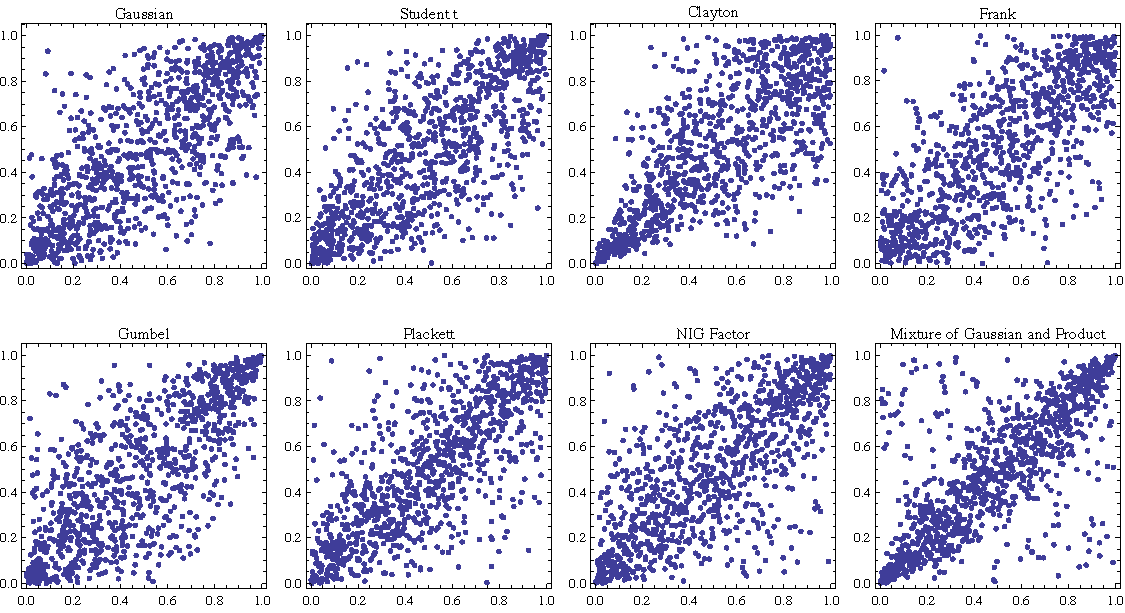
\includegraphics[width=\textwidth]{_pics/copulas_scatterplots.pdf}
  \caption{Scatterplots of samples drawn from copulae. All copulae are calibrated to Spearman's $\rho$ of 0.75 before sampling.}\label{fig:copulaeScatterPlot}
\end{figure}


\subsubsection{Gaussian and $t$ Copulae}\label{sec:ellpitical-copulae}

Gaussian and $t$ copulae are dervived from Gaussian and $t$ distributions.
Since Gaussian and $t$ distributions are elliptical distributions, Gaussian and $t$ copulae are called elliptical copulae.

Gaussian copula (bivariate) is defined as
\begin{align*}
  \bm{C}(u,v) &= \Phi_{2, \rho}\{\Phi^{(-1)}(u), \Phi^{(-1)}(v)\} \nonumber \\
              &= \int_{-\infty}^{\Phi^{(-1)}(u)}
                \int_{-\infty}^{\Phi^{(-1)}(v)}
                \frac{1}{2\pi\sqrt{1-\rho^2}}
                \exp{\left\{
                \frac{s^2-2\rho st+t^2}{2(1-\rho^2)}
                \right\}} \dd s\, \dd t,
\end{align*}
where $\Phi_{2, \rho}$ is the cdf of bivariate Normal distribution
with zero mean, unit variance, and correlation coefficient $\rho$, and
$\Phi^{(-1)}$ is the quantile function univariate standard normal
distribution.

Note that we use $\rho$ to denote the correlation parameter as well as a $\rho(\cdot)$ to denote a risk measure.

The Gaussian copula is fully specified by the correlation parameter $\rho$.
Like all elliptical copulas, it is symmetric.
It has no tail dependence, which, in a finance context, implies that it often underestimates tail risk.

The Gaussian copula density is
\begin{align*}
  \bm{c}_\rho(u,v) &= \frac{\bm{\varphi}_{2,\rho}\{\Phi^{(-1)}(u), \Phi^{(-1)}(v)\}}
                     {\varphi\{\Phi^{(-1)}(u)\} \cdot \varphi\{\Phi^{(-1)}(v)\}} \nonumber \\[10pt]
                   &= \frac{1}{2\pi\sqrt{1-\rho^2}}\exp\left\{
                     -\frac{u^2 - 2\rho uv + v^2}{2(1-\rho^2)}
                     \right\},
\end{align*}
where $\bm{\varphi}_{2,\rho}(\cdot)$ is the pdf corresponding to
$\Phi_{2, \rho}$, and $\varphi(\cdot)$ the standard normal
distribution pdf.

Kendall's $\tau_K$ and Spearman's $\rho_S$ of a bivariate Gaussian copula are
    \begin{align*}
        \tau_K(\rho) = \frac{2}{\pi}\arcsin\rho
        \end{align*}
    \begin{align*}
        \rho_S(\rho) = \frac{6}{\pi}\arcsin\frac{\rho}{2}.
        \end{align*}

The $t$-copula has the form
\begin{align*}
        \bm{C}(u,v) &= \bm{T}_{2, \rho, \nu}\{T^{(-1)}_\nu(u), T^{(-1)}_\nu(v)\} \nonumber \\[10pt]
            &= \int_{-\infty}^{T^{(-1)}_\nu(u)}
               \int_{-\infty}^{T^{(-1)}_\nu(v)}
            \frac{\Gamma\left(\frac{\nu+2}{2}\right)}
            {\Gamma\left(\frac{\nu}{2}\right)\pi\nu\sqrt{1-\rho^2}}\\[10pt]
           & \left(
        1+\frac{s^2-2st\rho+t^2}{\nu}
        \right)^{-\frac{\nu+2}{2}} ds dt,
    \end{align*}
where $\bm{T}_{2, \rho, \nu}$ denotes the cdf of
bivariate $t$ distribution with dependence parameter $\rho$ and degrees of freedom parameter $\nu$,
and where $T^{(-1)}_\nu(\cdot)$ is the quantile function of a standard
$t$ distribution with degree of freedom $\nu$.

Contrary to the Gaussian copula, the $t$-copula has a non-zero
tail dependence coefficient, which makes it more appropriate for
dependence modelling in finance. The Gaussian copula arises as
$\nu\rightarrow\infty$.

The copula density is
\begin{align*}
    \bm{c}(u,v) &= \frac{\bm{t}_{2, \rho, \nu}\{T^{(-1)}_\nu(u), T^{(-1)}_\nu(v)\}}
    {t_\nu\{T^{(-1)}_\nu(u)\}\cdot t_\nu\{T^{(-1)}_\nu(v)\}},
    \end{align*}
where $\bm{t}_{2,\rho, \nu}$ is the pdf of $\bm{T}_{2, \rho, \nu}$
and $t_\nu$ the density of standard $t$ distribution.

Like all the other elliptical copulae, the $t$-copula's Kendall's
$\tau$ is identical to that of the Gaussian copula \citep[see][and
references therein]{demarta2005t}.


\subsubsection{Archimedean copulae}\label{sec:archimedean-copula}
The family of Archimedean copulae forms a large class of copulae with
many convenient features.
Contrary to elliptical copulas, which are derived from
elliptical distributions.
Archimedean copulas are determined via a simple parametric form of the dependence structure.
A prominent feature is the ability to model asymmetric dependence structures.

In general, they take a form
\begin{align*}
    \bm{C}(u,v)= \psi^{(-1)}\{\psi(u), \psi(v)\},
    \end{align*}
where $\psi:[0,1] \rightarrow [0,\infty)$ is a continuous, strictly
decreasing and convex function such that $\psi(1)=0$ for any
permissible dependence parameter $\theta$. $\psi$ is also called
generator. $\psi^{(-1)}$ is the inverse of the generator.

The Frank copula (B3 in \citet{joe1997multivariate}) is a radial symmetric copula and cannot produce any tail dependence.
It takes the form
\begin{align*}
    \bm{C}_{\theta}(u,v) &= \frac{1}{\theta}
    \log \left\{
    1 + \frac{(e^{-\theta u}-1)(e^{-\theta v}-1)}{e^{-\theta}-1}
    \right\}
    \end{align*}
where $\theta \in [0, \infty]$ is the dependency parameter.
$\bm{C}_{-\infty} = \bm{M}$, $\bm{C}_1 = \bm{\Pi}$, and $\bm{C}_\infty = \bm{W}$.

The Copula density is
\begin{align*}
    \bm{c}_{\theta}(u,v) &= \frac{\theta e^{\theta(u+v)(e^\theta-1)}}
    {\left\{e^\theta-e^{\theta u}-e^{\theta v}+e^{\theta (u+v)}\right\}^2}
    \end{align*}

Frank copula has Kendall's $\tau$ and Spearman's $\rho$ as follow:
\begin{align*}
    \tau_K(\theta) = 1-4\frac{D_1\{-\log(\theta)\}}{\log(\theta)},
    \end{align*}
and
\begin{align*}
    \rho_S(\theta) = 1-12\frac{D_2\{-\log(\theta)\} - D_1\{\log(\theta)\}}{\log(\theta)},
    \end{align*}
where $D_1$ and $D_2$ are the Debye function of order 1 and 2.
Debye function is $D_n = \frac{n}{x^n}\int_0^x\frac{t^n}{e^t-1}dt$.

The Gumbel copula (B6 in \citet{joe1997multivariate}) has upper tail
dependence with the dependence parameter $\lambda^U =
2-2^{\frac{1}{\theta}}$ and displays no lower tail dependence.
\begin{equation*}
  \bm{C}_{\theta}(u,v) = \exp{-\{ (-\log(u))^\theta +(-\log(v))^\theta
    \}^{\frac{1}{\theta}}},
\end{equation*}
where $\theta \in [1,\infty)$ is the dependence parameter.

While the Gumbel copula cannot model perfect counter-dependence
\citep{Nelsen2002}, $\bm{C}_{1} = \bm{\Pi}$ models the independence,
and $\lim_\theta^\infty \bm{C}_\theta = \bm{W}$ models the perfect
dependence. The copula density takes the form
%\begin{align}
%        f
%    \end{align}
  \begin{equation*}
    \tau_K(\theta) =\frac{\theta-1}{\theta}.
   \end{equation*}

The Clayton copula, by contrast to Gumbel copula,
generates lower tail dependence of the form $\lambda^L =
2^{-\frac{1}{\theta}}$, but cannot generate upper tail dependence.
The Clayton copula takes the form
\begin{equation*}
  \bm{C}_{\theta}(u,v) = \left\{
    \max(u^{-\theta}+v^{-\theta}-1,0)\right\}^{-\frac{1}{\theta}},
\end{equation*}
where $\theta \in (-\infty, \infty)$ is the dependence parameter.
Moreover, $\lim_\theta^{-\infty} \bm{C}_\theta = \bm{M}$, $\bm{C}_0 =
\bm{\Pi}$, and $\lim_\theta^\infty \bm{C}_\theta = \bm{W}$.
Kendall's $\tau$ of the Clayton copula is given by
\begin{align*}
    \tau_K(\theta) =\frac{\theta}{\theta+2}.
    \end{align*}

\subsubsection{Mixture Copula}\label{sec:mixture-copula}
The mixture copula is a linear combination of copulae.
For a 2-dimensional random variable $\bm{X}=(X_1,X_2)^\top$,
its distribution can be written as linear combination of $K$ copulae

\begin{equation*}
    \bm{C}(u,v)= \sum_{k=1}^K p^{(k)} \cdot \bm{C}^{(k)}\{F^{(-1)}_{X_1}(u),
    F^{(-1)}_{X_2}(v); \bm{\theta^{(k)}}\}.
    \end{equation*}
The copula density is again a linear combination of copula densities
\begin{align*}
    \bm{c}(u,v)= \sum_{k=1}^K p^{(k)} \cdot \bm{c}^{(k)}\{F^{(-1)}_{X_1}(u),
    F^{(-1)}_{X_2}(v); \bm{\theta^{(k)}}\}.
    \end{align*}

While Kendall's $\tau$ of mixture copula is not known in closed form,
Spearman's $\rho$ is specified by the following statement.

\begin{proposition}
  Let $\rho_S^{(k)}$ be Spearman's $\rho$ of the $k$-th component
  Spearman's $\rho$ of the mixture copula is given by
  \begin{align*}
        \rho_S = \sum_{k=1}^K p^{(k)} \cdot \rho_S^{(k)}
        \end{align*}
    \end{proposition}

\begin{proof}
    Since Spearman's $\rho$ is defined as \citep{Nelsen1999}
    \begin{equation*}
      \rho_S = 12 \int_{\mathbb{I}^2} \bm{C}(s,t) ds dt - 3,
    \end{equation*}
    Spearman's $\rho$ of the the mixture copula is given by summation
    of the components
       \begin{align*}
        \rho_S = 12 \int_{\mathbb{I}^2} \sum_{k=1}^K p^{(k)} \cdot
         \bm{C}^{(k)}(s,t) ds dt - 3.
        \end{align*}
    \end{proof}

An example of a mixture copula is the Fr'echet class of copulas, which are given by convex combinations of $\bm{W}$,
  $\bm{\Pi}$, and $\bm{M}$ \citep{Nelsen1999}.

We use a mixture of Gaussian and independent copulas in our analysis,
i.e.,
\begin{equation*}
  \bm{C}(u,v) = p\cdot \bm{C}^\text{Gaussian}(u,v) + (1-p)(uv),
\end{equation*}
with corresponding density is
\begin{equation*}
  \bm{c}(u,v) = p\cdot \bm{c}^\text{Gaussian}(u,v) + (1-p).
\end{equation*}

This mixture models the amount of ``random noise'' that appears in the
dependence structure. In the hedging exercise, the
``random noise'' adds an unhedgable component to the two-asset portfolio, whose weight $(1-p)$ is calibrated from market data.

\subsubsection{NIG factor copula}

The {\em normal inverse Gaussian (NIG)\/} distribution, introduced by
\citep{BarndorffNielsen1997}, has density function
\begin{equation*}
  g(x; \alpha,\beta, \mu, \delta) = \frac{\alpha}{\pi} \e^{\delta
    \sqrt{\alpha^2-\beta^2} -\beta\mu} \frac{1}{q((x-\mu)/\delta)}
  K_1\left[\delta \alpha q\left(\frac{x-\mu}{\delta}\right) \right]
  \e^{\beta x},\quad x>0,
\end{equation*}
where $q(x) = \sqrt{1+x^2}$ and where $K_1$ is the modified Bessel
function of third order and index $1$. The parameters satisfy $0\leq
|\beta|\leq \alpha$, $\mu\in \R$ and $\delta>0$. The parameters have
the following interpretation: $\mu$ and $\delta$ are location and
scale parameters, respectively, $\alpha$ determines the heaviness of
the tails and $\beta$ determines the degree of asymmetry. If
$\beta=0$, then the distribution is symmetric around $\mu$.

The moment-generating function of the NIG distribution is given by
\begin{equation*}
  M(u; \alpha, \beta, \mu, \delta) = \exp\left( \delta
    \left(\sqrt{\alpha^2-\beta^2} - \sqrt{\alpha^2 - (\beta +
        u)^2}\right) + \mu u\right).
\end{equation*}
As a direct consequence, moments are easily calculated with the
expectation and variance of the NIG distribution being
\begin{align*}
  \mathbb E X &= \mu +
                \frac{\delta \beta}{\sqrt{\alpha^2-\beta^2}}
  \end{align*}
\begin{align} \label{eq:5}
  \text{Var}(X) &= \frac{\alpha^2\delta}{(\alpha^2-\beta^2)^{3/2}}.
\end{align}


The $\text{NIG}(\alpha, \beta, \mu\, \delta)$ distribution belongs to
the class of so-called {\em normal
variance-mean mixture},  (see Section 3.2 of
\citep{McNeil2005}): $X$ follows an
$\text{NIG}(\alpha,\beta,\mu,\delta)$ distribution if $X$ conditional
on $W$ follows a normal distribution with mean $\mu+\beta W$ and
variance $W$, i.e.,
\begin{equation*}
  X|W\stackrel{\mathcal L}\sim \Ncdf(\mu + \beta W, W),
\end{equation*}
where $W$ follows an {\em inverse Gaussian distribution}, denoted by
$\text{IG}(\delta, \sqrt{\alpha^2-\beta^2})$.

It is easily seen from the moment-generating function that the NIG distribution is preserved under linear combinations, provided
the variables share the parameters $\alpha$ and $\beta$. For this
and other reasons, the NIG distribution is popular in many areas of
financial modelling; for example, it gives rise
to the normal inverse Gaussian L\'evy process, which may be represented
as a Brownian motion with a time change.

In the setting here, we consider the {\em NIG factor copula}. This is
not directly derived from the multivariate NIG distribution, but
determined through a factor structure instead. The factor structure,
which
was applied e.g.\ in \citep{Kalemanova2007} for calibrating CDO's,
gives additionaly flexibility as it does not force the components to
have a mixing variable $W$.
The following proposition introduces the NIG factor model and some of
its properties.
\begin{proposition}
  \label{prop:NIG}
  Let $Z\sim \text{NIG}(\alpha, \beta, \mu, \delta)$ and
  $Z_i\sim \text{NIG}(\alpha, \beta, \mu_i, \delta_i)$,
  $i=1,\ldots, n$ be independent NIG-distributed random
  variables. Then:
  \begin{enumerate}
  \item  $X_i = Z + Z_i\sim \text{NIG}(\alpha,\beta,\mu+\mu_i,
  \delta+\delta_i)$,
\item and
  \begin{align}
    \text{Cov}(X_i,X_j) &= \text{Var(Z)},\nonumber\\
    \text{Corr}(X_i,X_j) &= \frac{\delta}{\sqrt{(\delta+\delta_i)
                           (\delta+\delta_j)}}. \label{eq:6}
  \end{align}
\end{enumerate}
\end{proposition}
\begin{proof}
  \begin{enumerate}
  \item This follows directly from the moment-generating function.
  \item For the covariance,
    \begin{align*}
      \text{Cov}(X_i,X_j)
      &= \E[(Z+Z_i) (Z+Z_j)] - \E[Z+Z_i] \E[Z+Z_j]\\
      &= \E[Z^2] -(\E Z)^2.
    \end{align*}
    The correlation is determined directly from \ref{eq:5}.
  \end{enumerate}
\end{proof}

The NIG factor copula is obtained by transforming the margins to
uniforms (see Sklar's Theorem), giving (e.g.\
\citep{krupskii2013factor}):
\begin{equation*}
  C_{r^S, r^F}(F_{r^S}(r^S), F_{r^F}(r^F)) = \int_\mathbb{R}
  F_{Z_1}(F_{X_1}^{(-1)} \circ F_{r^S}(r^S) -z) \cdot
  F_{Z_2}(F_{X_2}^{(-1)} \circ F_{r^F}(r^F) -z) \cdot
  f_Z(z) dz
  \end{equation*}
If the margins are continuous, then Spearman's rho of NIG factor
copula is
\begin{equation*}
  \rho_S = 12 \int \int \int_{\mathbb{R}^3}
  F_{X_1}(x_1) \cdot
  F_{X_2}(x_2) \cdot
  f_{Z_1}(x_1-z) \cdot
  f_{Z_2}(x_2-z) \cdot
  f_Z(z) dx_1 dx_2 dz - \frac{1}{48}.
  \end{equation*}

% \begin{proof}
%   \begin{align}
%   \rho_S(r^S, r^F) &= \rho\{F_{r^S}(r^S), F_{r^F}(r^F)\} \\
%     &= \rho\{F_{X_1}(X_1), F_{X_2}(X_2)\} \\
%     &= 12 \cdot \mathbb{E}\{F_{X_1}(X_1) \cdot F_{X_2}(X_2) \} - \frac{1}{48}\\
%     &= 12 \cdot \int \int_{\mathbb{R}^2} F_{X_1}(X_1) \cdot F_{X_2}(X_2) dF_{X_1,X_2}(x_1,x_2)\\
%     \end{align}
%   Because
%   \begin{align}
%     F_{X_1,X_2}(x_1,x_2) &= \mathbb{P}(X_1 \leq x_1, X_2 \leq x_2)\\
%     &= \mathbb{P}(Z_1 \leq x_1 - Z, Z_2 \leq x_2 - Z) \\
%     &= \int_\mathbb{R}\mathbb{P}(Z_1 \leq x_1 - z) \cdot \mathbb{P}(Z_2 \leq x_2 - z) \cdot f_Z(z) dz,
%     \end{align}
%   so,
%   \begin{align}
%     \rho_S(r^S, r^F) = 12 \cdot \int \int \int_{\mathbb{R}^3} F_{X_1}(x_1) \cdot F_{X_2}(x_2) \cdot f_{Z_1}(x_1 -z) \cdot f_{Z_2}(x_2 -z) \cdot f_{Z}(z) dx_1 dx_2 dz -\frac{1}{48}
%     \end{align}
%   \end{proof}


\subsubsection{Plackett copula}\label{subsec:other-copula}
The Plackett copula has an expression
\begin{align*}
    \bm{C}_{\theta}(u,v) &= \frac{1+(\theta-1)(u+v)}{2(\theta-1)}
                         - \frac{\sqrt{\{
    1+(\theta-1)(u+v)\}^2 - 4uv\theta(\theta-1)}}{2(\theta-1)}
    \end{align*}
\begin{align*}
    \rho_S(\theta) = \frac{\theta+1}{\theta-1} - \frac{2\theta \log \theta}{(\theta-1)^2}
    \end{align*}

We include Placket copula in our analysis as it possesses a special property,
the cross-product ratio is equal to the dependence parameter
\begin{align} \label{eq:PlackettCrossProduct}.
    &\phantom{=} \frac{\p(U \leq u, V \leq v) \cdot \p(U > u, V > v)}
    {\p(U \leq u, V > v) \cdot \p(U > u, V \leq v)}\nonumber\\
    &= \frac{\bm{C}_\theta(u,v)\{1-u-v+\bm{C}_\theta(u,v)\}}{\{u-\bm{C}_\theta(u,v)\}\{v-\bm{C}_\theta(u,v)}\nonumber\\
    &= \theta.
    \end{align}

That is, the dependence parameter is equal to the ratio between number of concordence pairs and number of discordence pairs of a bivariate random variable.

%! Author = francis
%! Date = 30.10.20

\subsection{Calibration and selection of copulae}\label{sec:estimation}
We introduce the method to calibrate copulae to our data in this section.
In general, there are two types of calibration procedures to calibrate copulae:
maximum likelihood (MLE) and method of moments (MM).
We decide to deploy the latter since it calibrates according to the moments desired.

In the following subsection, we present the configuration of the method of moments procedures in this work.
In the subsection after, we argue that MM is more suitable to this work by comparing MM with MLE.

\subsubsection{Method of moments}
\label{subsec:simulated-method-of-moments}

We trace back the usage of MM to calibrate copulae to \citet{Genest1987, genest1993statistical}.
The moments mainly refer to Kendall's $\tau$ or Spearman's $\rho$.
We extend MM to quantile dependence measures denoted by $\lambda_q$ for quantile level $q$.

Spearman's $\rho$, Kendall's $\tau$, and quantile dependence of the copula $C$ are defined as
\begin{align*}
  \rho_S &= 12 \int\int_{I^2} C_{\bm{\theta}}(u,v)\, \dd u\, \dd v-3\label{eq:rho_S}\\
  \tau_K &= 4\E[C_{\bm{\theta}}\{F_X(x), F_Y(y)\}]-1,\\
  \lambda_q &=
  \begin{cases}
    \p(F_X(X)\leq q| F_Y(Y)\leq q) = \displaystyle \frac{C_{\bm{\theta}}(q,q)}{q},
    &\text{ if } q\in (0,0.5],\\
    \p(F_X(X)>q|F_Y(Y)>q) =\displaystyle \frac{1-2q+C_{\bm{\theta}}(q,q)} {1-q},
    &\text{ if } q\in (0.5,1).
  \end{cases}
\end{align*}
The empirical counterparts are
\begin{align*}
  \hat\rho_S &= \frac{12}{n} \sum_{k=1}^n \hat F_X(x_k) \hat F_Y(y_k)
               -3,\\
  \hat\tau_K &= \frac{4}{n}\sum_{k=1}^n \hat{C}\{\hat{F}_X(x_i),\hat{F}_X(y_i)\} -1 ,\\
  \hat\lambda_q &=
                  \begin{cases}
                    \displaystyle\frac{1}{n} \sum_{k=1}^n \frac{\1_{\{\hat
                        F_X(x_k)\leq q, \hat F_Y(y_k)\leq q\}}} {q},
                    &\text { if } q\in (0, 0.5],\\
                    \displaystyle \frac{1}{n} \sum_{k=1}^n
                    \frac{\1_{\{\hat F_X(x_k)>q, \hat F_Y(y_k)>q\}}}
                    {1-q}, &\text { if } q\in (0.5,1),
                  \end{cases}
\end{align*}
where $\displaystyle \hat{F}(x) =
  \frac{1}{n}\sum_{k=1}^n 1_{\{x_i\leq x\}}$ and
$\displaystyle \hat{C}(u,v) = \frac{1}{n}\sum_{k=1}^n 1_{\{u_i\leq u, v_i\leq v\}}$.

Denote by $\bm{m}(\bm{\theta})$ the $m$-dimensional vector of
dependence measures according the dependence parameters
$\bm{\theta}$,and let $\hat{\bm{m}}$ be the corresponding empirical
counterpart.
The difference between dependence measures and their counterpart is denoted by
\begin{align*}
    \bm{g}(\bm{\theta}) = \hat{\bm{m}} - \bm{m}(\bm{\theta}).
\end{align*}

The MM estimator is
\begin{align*}
    \hat{\bm{\theta}} = \argmin_{\bm{\theta}\in \bm{\Theta}} \bm{g}(\bm{\theta})^\top
    \hat{\bm{W}}
     \bm{g}(\bm{\theta}),
\end{align*}
where $\hat{W}$ is some positive definite weight matrix.
In this work, we use
$\bm{m}(\bm{\theta}) = (\rho_S, \lambda_{0.05}, \lambda_{0.1},
\lambda_{0.9}, \lambda_{0.95})^\top$
for calibration.
$\hat{W}$ is set to identity matrix.

\subsubsection{Comparison between method of moments and maximum likelihood}
\label{subsec:maximum-likelihood-estimation}
By the Hoeffding-Sklar theorem, the joint density of a $d$-dimensional random variable $\bm{X}$ with sample size $n$ can be written as
\begin{equation*}
    \bm{f}_{\bm{X}}(x_1, ..., x_d) = \bm{c}\{F_{X_1}(x_1), ..., F_{X_d}(x_d)\} \prod_{j=1}^d f_{X_i}(x_i).
    \end{equation*}
We follow the treatment of MLE documented in section 10.1 of
\citet{joe1997multivariate}, namely the {\em inference functions for
margins (IFM) method}.
The log-likelihood $\sum^n_{i=1}f_{\bm{X}}(X_{i,1}, ..., X_{i,d})$ can be decomposed into a dependence part and a marginal part,
\begin{align*}
    L(\bm{\theta}) &= \sum_{i=1}^n \bm{c}\{F_{X_1}(x_{i,1};\bm{\delta}_1), ..., F_{X_d}(x_{i,d}; \bm{\delta}_d);\bm{\gamma}\}
    + \sum_{i=1}^n \sum_{j=1}^d f_{X_j}(x_{i,j};\bm{\delta}_j)\\
    &= L_C(\bm{\delta}_1, ..., \bm{\delta}_d, \bm{\gamma}) + \sum_{j=1}^d L_j(\bm{\delta}_j)
    \end{align*}
where $\bm{\delta}_j$ are the parameters of the $j$-th margin, $\bm{\gamma}$ is the parameter of the parametric copula, and
$\bm{\theta} = (\bm{\delta}_1,..., \bm{\delta}_d, \bm{\gamma})$.
Instead of searching the $\bm{\theta}$ in a high dimensional space, \citet{joe1997multivariate} suggests to
search for $\hat{\bm{\delta}_1},..., \hat{\bm{\delta}_d}$ that maximize $L_1(\bm{\delta}_1), ..., L_d(\bm{\delta}_d)$,
then search for $\hat{\bm{\gamma}}$ that maximize $L_C(\hat{\bm{\delta}_1},..., \hat{\bm{\delta}_d}, \bm{\gamma})$.

%\natp{\em [I suggest to delete the next part, as the regularity
%  conditions are unclear, and it is just a first-order condition,
%  which is a-priori not clear to hold in a two-step procedure.]}
%That is, under regularity conditions, $(\hat{\bm{\delta}_1},..., \hat{\bm{\delta}_d}, \hat{\bm{\gamma}})$ is the solution of
%\begin{align}
%    \left( \frac{\partial L_1}{\partial \bm{\delta}_1}, ..., \frac{\partial L_d}{\partial \bm{\delta}_d},
%    \frac{\partial L_C}{\partial \bm{\gamma}}\right) = \bm{0}.
%    \end{align}

%However, the IFM requires making assumption on the distribution of the
%margins.\natp{\em [delete until here.]}

We follow \citet{genest1995semiparametric} who suggest to replace the estimation of marginals parameters estimation by non-parameteric estimation.
Given non-parametric estimator $\hat{F}_i$ of the margins $F_i$, the estimator of the dependence parameters $\bm{\gamma}$ is
\begin{equation*}
    \hat{\bm{\gamma}} = \argmax_{\bm{\gamma}} \sum_{i=1}^n \bm{c}\{ \hat{F}_{X_1}(x_{i,1}), ..., \hat{F}_{X_d}(x_{i,d});\bm{\gamma}\}.
    \end{equation*}

Both the simulated method of moments and the maximum likelihood estimation are unbiased.
The question though which procedure is more suitable for hedging.

\begin{figure}[h]
%\includegraphics[width=\textwidth]{_pics/t Copula quantile dependence.png}
\includegraphics[width=\textwidth]{_pics/Gumbel Copula quantile dependence.pdf}
\includegraphics[width=\textwidth]{_pics/Clayton Copula quantile dependence.pdf}
  \caption{Quantile dependences of Gumbel, and Clayton Copula. The \textcolor{darkblue}{blue circle dots} are
  the quantile dependence estimates of Bitcoin and CME future, \textcolor{darkblue}{blue dotted lines} are the estimates' 90\% confidence interval.
  \textcolor{orange}{Orange dotted line} is the copula implied quantile dependence by MM estimation.
  \textcolor{lightblue}{Light blue dotted line} is the copula implied quantile dependence by MLE estimation.
%  \href{http://www.quantlet.com/}{\includegraphics[height=\baselineskip]{_pics/qletlogo_tr.png}}
  }
\label{fig:quantile dependence1}
\end{figure}

Figure~\ref{fig:quantile dependence1} shows the empirical quantile dependence of Bitcoin and CME future and the copula implied
quantile dependence of the MLE and MM calibration procedures.
Although the MLE is a better fit to a range of quantile dependence in the middle, it fails to address the situation in the tails.
We find that our data empirically has low quantile dependence in the lower ends ($q<10\%$).
We argue that MM is preferred as it produces a better fit to the dependence
structure in the tail behaviour, contrary to MLE.

Therefore, we deploy the method of moments throughout the
analysis.
We choose the $5^\text{th}$-, $10^\text{th}$-, $90^\text{th}$-, $95^\text{th}$-quantile, and Spearman's $\rho$ as the moments.


\subsubsection{Copula selection}\label{subsec:copula-selection}
The dependence structure of price data changes across time, in which
both the dependency parameters and the type of dependence.
For this reason, we allow for a flexible choice of the best-fitting copula, by re-calibrating periodically and re-evaluating performance of the various copulas.
We select the best-fitting copula, characterised by the lowest {\em Akaike Information Criterion (AIC)},
\begin{equation*}
 \text{AIC} = 2k- 2 \log(L),
\end{equation*}
where $k$ is the number of estimated parameters and $L$ is the likelihood \citep{Akaike1973}.

Other model selection criteria, such as the TIC~\citep{takeuchi1976distribution} or likelihood ratio test could be used instead.
For a survey of model selection and inference, see \cite{anderson1998comparison}.
Among various copula selection procedures, AIC is a popular choice for
its applicability, see e.g. \cite{breymann2003dependence}.
In our case, the AICs are calculated only with dependency likelihood
since the marginals are modelled via kernel density estimators.
The selected copula will then be enter the calculation of the optimal
hedge ratio.

\subsection{Risk measures}\label{subsec:spectral-risk-measures}
The optimal hedge ratio is determined for the following variety of risk measures: variance, Value-at-Risk (VaR), Expected Shortfall (ES), and Exponential Risk Measure (ERM).
A summary of risk measures being used in portfolio selection problem
can be found in \citet{hardle2008applied}.
The risk measures here serve as risk minimization objectives, i.e. loss functions for searching the optimal hedge ratio.

The risk measures are defined as follows.
Let $Z$ be a random
variable with distribution function $F_Z$.
\begin{enumerate}
\item Variance: $\text{Var}(Z) = \E[(Z-\E Z)^2]$.
\item VaR at confidence level $\alpha$: $\text{VaR}_\alpha(Z) = -F_{Z}^{(-1)}(1-\alpha)$
\item ES at confidence level $\alpha$: $\text{ES}(F_Z) = -\frac{1}{1-\alpha}\int_0^{1-\alpha}F_Z^{(-1)}(p)dp$
\item ERM with Arrow-Pratt coefficient of absolute risk
  aversion $k$:
  \begin{equation*}
    \text{ERM}_k(F_Z) = \int_0^{1-\alpha}\phi(p) F_Z^{(-1)}(p)dp,
  \end{equation*}
  where $\phi$ is a weight function described in (\ref{eq:phi}) below.
\end{enumerate}

VaR, ES, and ERM fall into the class of spectral risk measures (SRM),
which have the from \citep{Acerbi2002}%, adam2008spectral,dowd2008spectral}
\begin{equation*}
  \rho_\phi(r^h) = - \int_0^1 \phi(p) F_{Z}^{(-1)}(p)d p,
\end{equation*}
where $p$ is the loss quantile and $\phi(p)$ is a user-defined
weighting function defined on $[0,1]$.
We consider only so-called admissible risk spectra $\phi(p)$, i.e.,
fulfilling %(named by \citet{Acerbi2002})
\begin{enumerate}[label=(\roman*)]
\item $\phi$ is positive,
\item $\phi$ is decreasing,
\item and $\int\phi=1$.
\end{enumerate}

The VaR's $\phi(p)$ gives all its weight on the $1-\alpha$ quantile of $Z$ and zero elsewhere,
i.e. the weighting function is a Dirac delta function, and hence it
violates the (ii) property of admissible risk spectra.
The ES' $\phi(p)$ gives all tail quantiles the same weight of
$\displaystyle\frac{1}{1-\alpha}$ and non-tail quantiles zero weight.
The ERM assumes investors' risk preference are in the form of an
exponential utility function $U(x)=1-e^{kx}$, so its corresponding
risk spectrum is defined as
\begin{equation*}
  \phi(p) =\frac{k e^{-k(1-p)}}{1-e^{-k}} , \label{eq:phi}
\end{equation*}
where $k$ is the Arrow-Pratt coefficient of absolute risk aversion.
The parameter $k$ has an economic interpretation as being the ratio
between the second derivative and first derivative
of investor's utility function on an risky asset,
\begin{equation*}
  k = -\frac{U''(x)}{U'(x)},
\end{equation*}
for $x$ in all possible outcomes.
In case of the exponential utility, $k$ is the the constant absolute risk aversion (CARA).

\newpage
%
\bibliography{finance} %
\end{document}


%%% Local Variables:
%%% mode: latex
%%% TeX-master: "SRM"
%%% End: